\section{Theorie}
\label{sec:Theorie}
\subsection{Einleitung}
Mittels der Kernspinresonanz können Spins in einem homogenen Magnetfeld mit Hochfrequenzfeld beeinflusst werden. In diesem Versuch werden die Spins einer destillierten Wasser-Probe aus ihrem Gleichgewicht gebracht, wodurch spezifische Relaxationszeiten und die Diffusionskonstante bestimmt werden können.
\subsection{Allgemeine Grundlagen}
\subsubsection{Magnetisierung im thermischen Gleichgewicht}
Wird ein externes Magnetfeld an eine Probe angelegt, beispielsweise parallel zur z-Richtung, entsteht eine makroskopische Magnetisierung der Probe. Dieses tritt auf, da die Kernspinzustände entarten und somit sich die einzelnen magnetischen Momente orientieren. Bei einem Proton mit Kernspin $I=\frac{1}{2}$ existieren, aufgrund des Zeemaneffekts, zwei Unterniveaus mit der magnetischen Quantenzahl $m=-\frac{1}{2}$ und $m=\frac{1}{2}$. Anhand der Maxwell-Boltzmann-Statistik kann eine Aussage über Besetzung der beiden Unterniveaus getroffen werden. Bei Betrachtung im thermischen Gleichgewicht fällt bei dem Besetzungsverhältnis der beiden Zustände
\begin{align}
	\frac{N(m)}{N(m-1)}=\exp{\left(\frac{\Delta E}{k_BT}\right)}
	\label{eq:verhaeltniss}
\end{align}
auf, dass die Niveaus nur leicht unterschiedlich besetzt sind, da bei sehr hohen Temperaturen das Verhältnis gegen 1 kovergiert. Aus der ungleichen Besetzung resultiert eine Kernspinpolaritation, wodurch sich aus den einzelnen magnetischen Momenten $\mu_i$ eine makroskopische Gesamtmagnetisierung der Probe 
\begin{align}
	M_0 = \frac{1}{4}\mu_0\gamma^2\frac{\hbar^2}{k_B}N\frac{B_0}{T}
	\label{eq:gleichgewicht}
\end{align}
einstellt. Dabei steht $\mu_0$ für die Permeabilität des Vakuums, $\gamma$ für das gyromagnetische Verhältnis und N für die Anzahl der magnetischen Momente pro Volumeneinheit.

\subsubsection{Lamor-Präzession und Relaxationszeiten}
Wird durch Einstrahlung von Hochfrequenzquanten der Übergang in das höhere Niveau ermöglicht, entsteht ein Ungleichgewicht im Besetzungsverhältnis. Dadurch wirkt ein Drehmoment $D$ welches zu Präzessionsbewegung um die z-Achse führt. In einem Ein-Teilchen-System wird die Präzession mit der Kreisfrequenz 
\begin{align}
	\omega_L=\gamma B_0 \:,
	\label{eq:Lamor}
\end{align}
der sogenannten Lamorfrequenz, unendlich lange fortgesetzt. Wird jedoch ein Viel-Teilchen-System betrachtet, relaxiert der Spin aufgrund von Wechselwirkungen zurück in sein Gleichgewichtszustand. Die vorliegende Dynamik wird durch die Blochschen Differentialgleichungen beschrieben:
\begin{align}
	\frac{\text{d}M_z}{\text{d}t}&=\frac{M_0-M_z}{T_1}\\
	\frac{\text{d}M_x}{\text{d}t}&=\gamma B_0 M_y -\frac{M_x}{T_2}\\
	\frac{\text{d}M_y}{\text{d}t}&=\gamma B_0 M_x -\frac{M_y}{T_2}
	\label{eq:Bloch}
\end{align}
Die Relaxtionszeit $T_1$ wird auch longitudinale oder Spin-Gitter-Relaxationszeit genannt. Zum einen beschreibt sie also Veränderung parallel zur Feldrichtung und zum anderen die Zeit die benötigt wird bis freigewordene Kernspinenergie in Gitterschwingungen umgesetzt sind. Im Gegensatz dazu wird $T_2$ als transversale oder Spin-Spin-Relaxationszeit bezeichnet, da diese Veränderungen senkrecht zum anliegenden Feld beschreibt und verantwortlich ist für die Abnahme der senkrechten Magnetisierung, die durch Spin-Wechselwirkungen zustande kommen.

\subsubsection{HF-Einstrahlungsvorgänge und Pulse}
Zur Bestimmung der Zeitkonstanten wird ein HF-Feld senkrecht zur Probe angelegt. Weiterhin sei die Magnetfeld parallel zur z-Achse ausgerichtet, sodass gilt:
\begin{align}
	\vec{B}_{HF}=2\vec{B}_1 \cos{(\omega t)}
	\label{eq:8}
\end{align}
Das HF-Feld, aufgeteilt in zwei zirkular polarisierte Felder, rotiert mit der Frequenz $\omega$ und $-\omega$. Gilt $\omega_L \approx \omega$, so ist der Betrag von $-\omega$ zu vernachlässigen. Durch einen Koordinatenwechsel in das rotierende System, ist für den Beobachter im System das $B$-Feld kostant und die Einheitsvektoren zeitabhängig. Somit führt die Magnetisierung eine Präzession um die $B_1$-Achse aus. Beträgt die Einstrahlungszeit des HF-Feldes nun $\Delta t_{90}=\frac{\pi}{2\gamma B_1}$, verschwindet die z-Komponente, was bedeutet, dass die Magenetisierung in die $x$-$y$-Ebene gedreht wurde. Ein weiter $\Delta t_{180}=\frac{\pi}{\gamma B_1}$ Puls führt dazu, dass die Magnetisierung in die -$z$-Richtung klappt.

\subsection{Bestimmung der Spin-Gitter Relaxationszeit $T_1$}
Zur Bestimmung von $T_1$ wird zuerst ein \SI{180}{\degree}-Puls genutzt, der die Magnetisierung aus ihrer parallelen Lage zum $B$-Feld  in eine antiparallele Ausgangslage versetzt. Trotz des Impulses existiert weiterhin nur eine z-Komponente. Erst nach einer Zeit $\tau$, in der die Magnetisierung langsam wieder in Richtung ihrer Ausgangslage relaxiert, erhält diese auch $x$- und $y$-Komponenten. Durch einen  \SI{90}{\degree}-Puls wird dann die sich verkleinerne $z$-Komponente in die x-y-Ebene projeziert, wodurch in die HF erzeugende Spule (siehe Kapitel \ref{sec:Versuchaufbau}) eine Spannung induziert wird. Mit den Blochschen Gleichungen ergibt sich somit die zeitabhängige Magnetisierung
\begin{align}
	M(\tau)=M_0(1-2\exp{(-\tau/T_1)}) \: .
	\label{eq:30}
\end{align}
In Abbildung \ref{fig:plot1} ist der Verlauf der zuvor beschriebenen Gleichung dargestellt.

% % Standard Plot
\begin{figure}[H]
  \centering
  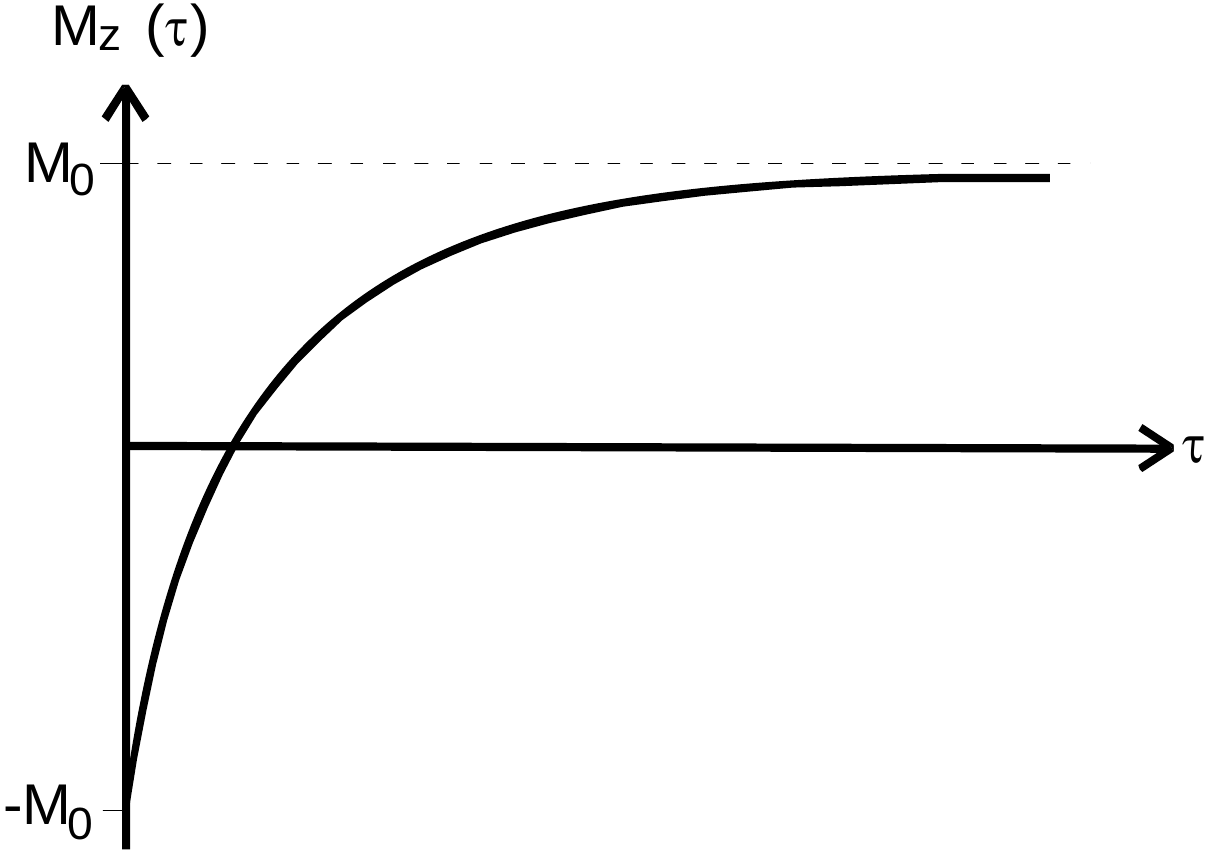
\includegraphics[width=0.475\textwidth]{ressources/T_1_plot.png}
  \caption{Verlauf der Relaxationszeit $T_1$.}
  \label{fig:plot1}
\end{figure}

\subsection{Bestimmung der Spin-Gitter Relaxationszeit $T_2$}
\subsubsection{Freie Induktion}
Die Magnetisierung wird durch einen $\Delta t_{90}$-Puls aus der Gleichgewichtlage in die x-y-Ebene gelengt, in der die Präzessionsbewegung eine Induktionsspannung in der probenumschließenden Spule erzeugt. Von da aus relaxiert diese wieder in ihre Ausgangslage zurück. Dieser Vorgang wird als Freie Induktion (FID) bezeichnet. Mit diesem Verfahren kann jedoch nicht zur Bestimmung von $T_2$ verwendet werden, da es zu einer Dephasierung der Spins kommt. Grund dafür ist zum einen die Dipolwechselwirkungen zwischen nächsten Nachbarn und zum andere die Inhomogenität der Polschuhe, wodurch die Spins schneller oder langsamer als die Lamorfrequenz rotieren.

\subsubsection{Spin-Echo-Verfahren}
Dieses Verfahren baut auf der freien Induktion auf, jedoch wird durch einen weiteren HF-Puls der Dephasierung entgegen gewirkt. Zu Beginn wird die Magnetisierung erneut mit einem $\Delta t_{90}$-Puls in die x-y-Ebene ausgelengt, in der die Spins beginnen mit leicht unterschiedlichen Frequenzen und Umlaufrichtungen zu rotieren. Nach einer Zeit $T$ ist die Auffächerung der Spins so groß, dass in der Spule kein Induktionssignal gemessen werden kann. Nach dem Zeitraum $\tau$  wird ein $\Delta t_{180}$-Puls genutzt um die Spins um \SI{180}{\degree} zu drehen. Somit laufen die Spins ab diesem Zeitpunkt wieder zusammen. Die Spins die zuvor mit einer im Betrag höheren Frequenz umgelaufen sind, haben ebenfalls eine längere Strecke in selber Zeit zurückgelegt, wie die langsameren Spins. Nach einem weiteren Zeitraum $\tau$ sind somit alle Spins für einen Augenblick in Phase und induzieren eine Spannung. Der zuvor beschriebene Ablauf ist in Abbildung \ref{fig:plot2} graphisch dargestellt. 


\begin{figure}
  \centering
  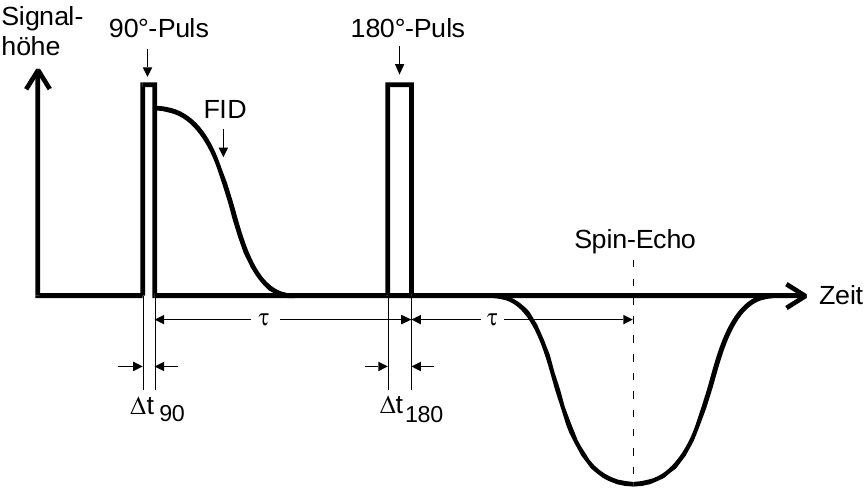
\includegraphics[width=0.75\textwidth]{ressources/hahn_echo.png}
  \caption{Skizze des Spin-Echo-Verfahrens.}
  \label{fig:plot2}
\end{figure}

Der Nachteil der Methode besteht darin, dass bei größerem Impulsabstand $\tau$ die Echosignalamplitude sinkt. Verursacht wird dieses durch die Dephasierung. Nach dem ersten $\Delta t_{90}$-Puls treten irreversible Dephasierungen durch Spinwechselwirkungen auf, die somit das Echosignal vermindern. Durch die Variation von $\tau$ und der Beziehung
\begin{align}
	M_y(t)=M_0\exp{(-t/T_2)} \:,
	\label{eq:11}
\end{align}
die die Echoamplitude in Abhängigkeit des Pulsabstand beschreibt, ist $T_2$ zu bestimmen.

Ein weiterer Nachteil besteht darin, dass es erforderlich ist nach jeder Echo-Messung zu warten, bis die Gleichgewichtsmagnetiesierung wieder hergestellt ist. Dies führt zu Wartezeiten im Sekundenbereich.

\subsubsection{Carr-Purcell- und Meiboom-Gill-Methode}
Die Carr-Purcell-Methode verringert die zuvor beschriebene Wartezeit, indem nach dem initialen $\Delta t_{90}$-Puls in $2\tau$-Abständen mehrere $\Delta t_{180}$-Pulse verwendet werden. Die Zeitkonstante $T_2$ kann somit erneut mit Gleichung \eqref{eq:11} bestimmt werden. Der Nachteil der Methode besteht darin, dass bei nicht exakter Justage des $\Delta t_{180}$-Pulses die Spins bei jedem Puls ein wenig aus der $x$-$y$-Ebene verschoben werden, sodass sich der Fehler nach und nach aufaddiert. Schlussendlich führt dieses zu einer zu kleinen Zeitkonstante $T_2$.

Um diesen Fehler zu kontrollieren und die Addition des selbigen zu verhindern kann die Meiboom-Gill-Methode verwendet werden. Der Unterschied zur Carr-Purcell-Methode besteht darin, dass die $\Delta t_{180}$-Pulse um \SI{90}{\degree} phasenverschoben werden im Gegensatz zum $\Delta t_{90}$-Puls. Die Drehungen finden somit in der y-Ebene statt. Der Fehler $\delta$ der beim ersten $\Delta t_{180}$-Puls verursacht wird, wird durch den zweiten korrigiert und somit die Spins zurück in die $x$-$y$-Ebene verlagert. Somit spiegelt jedes zweite Echo die korrekte, nicht fehlerbehaftete Höhe wieder.

\subsubsection{Einfluss der Diffusion auf die Bestimmung von $T_2$}
In Flüssigkeiten kommt es zur Diffusion infolge von brownscher Molekularbewegung. Diese verursacht, dass die Spins sich aufgrund der inhomogenen Magnetfeldstärke in andere Bereiche bewegen. Somit wird die Lamorfrequenz ortabhängig und das Spinecho nimmt schneller ab. Durch Berücksichtigung der Diffusion ergibt sich
\begin{align}
	M_y(t)=M_0\exp{(-t/T_2)}\exp{(-1/12D\gamma^2G^2t^3)} \:,
	\label{eq:32}
\end{align}
wobei G den Feldgradienten wiederspiegelt. Um die Gültigkeit der Formel zu gewährleisten ist sicherzustellen, dass die Diffusionszeit groß gegen die Relaxationszeit $T_2$ gewählt wird. Um die Diffusionskonstante $D$ zu bestimmen muss gelten
\begin{align}
	T_3^2 >>\frac{12}{D\gamma^2G^2},
	\label{eq:34_1}
\end{align}
sodass der Diffusionsterm in Gleichung \eqref{eq:32} dominiert.

% 2x2 Plot
% \begin{figure*}
%     \centering
%     \begin{subfigure}[b]{0.475\textwidth}
%         \centering
%         \includegraphics[width=\textwidth]{Abbildungen/Schaltung1.pdf}
%         \caption[]%
%         {{\small Schaltung 1.}}
%         \label{fig:Schaltung1}
%     \end{subfigure}
%     \hfill
%     \begin{subfigure}[b]{0.475\textwidth}
%         \centering
%         \includegraphics[width=\textwidth]{Abbildungen/Schaltung2.pdf}
%         \caption[]%
%         {{\small Schaltung 2.}}
%         \label{fig:Schaltung2}
%     \end{subfigure}
%     \vskip\baselineskip
%     \begin{subfigure}[b]{0.475\textwidth}
%         \centering
%         \includegraphics[width=\textwidth]{Abbildungen/Schaltung4.pdf}    % Zahlen vertauscht ... -.-
%         \caption[]%
%         {{\small Schaltung 3.}}
%         \label{fig:Schaltung3}
%     \end{subfigure}
%     \quad
%     \begin{subfigure}[b]{0.475\textwidth}
%         \centering
%         \includegraphics[width=\textwidth]{Abbildungen/Schaltung3.pdf}
%         \caption[]%
%         {{\small Schaltung 4.}}
%         \label{fig:Schaltung4}
%     \end{subfigure}
%     \caption[]
%     {Ersatzschaltbilder der verschiedenen Teilaufgaben.}
%     \label{fig:Schaltungen}
% \end{figure*}
